% ============================================================
\chapter{Bifurcations}
\label{ch:bifurcations}
% ============================================================

Imagine a physical system that depends on a parameter: the load on a bridge, the temperature of a fluid, the birth rate of a population. As the parameter varies, the system's behaviour changes gradually---until a critical threshold where everything shifts: a stable equilibrium disappears, a limit cycle appears, the number of solutions changes abruptly. This sudden qualitative change is a \emph{bifurcation}, and its classification---saddle-node, transcritical, pitchfork, Hopf---constitutes one of the most beautiful chapters in dynamical systems theory, inherited from Poincar\'e's work and systematised by Ren\'e Thom in his \emph{catastrophe theory} (1972).

\section{Introduction}

A \textbf{bifurcation} occurs when the qualitative structure of a dynamical
system's phase portrait changes as a parameter varies. This chapter studies
the most fundamental local bifurcations: saddle-node, transcritical,
pitchfork, and Hopf.

\section{General Framework}

\begin{definition}[Bifurcation]
Consider the parametric system $\dot{x} = f(x, \mu)$, where $x \in \R^n$
and $\mu \in \R^p$ is a parameter vector. A value $\mu_0$ is a
\textbf{bifurcation value} if the phase portrait of $f(\cdot, \mu)$ is not
topologically equivalent for $\mu$ near $\mu_0$ on either side.
\end{definition}

\begin{definition}[Local bifurcation]
A bifurcation is \textbf{local} if it is associated with the change of
stability of an equilibrium point, i.e., an eigenvalue of the Jacobian
crossing the imaginary axis.
\end{definition}

\begin{definition}[Codimension]
The \textbf{codimension} of a bifurcation is the minimum number of
independent parameters needed to observe it generically.
\end{definition}

\section{Saddle-Node Bifurcation}

\begin{definition}[Saddle-node bifurcation]
The \textbf{saddle-node bifurcation} (or \textbf{fold}) is the creation or
annihilation of two equilibrium points as a parameter crosses a critical value.
\end{definition}

\begin{theorem}[Saddle-node normal form]
\label{thm:saddle-node}
The normal form of the saddle-node bifurcation in dimension 1 is
\[
    \dot{x} = \mu + x^2.
\]
\begin{itemize}
    \item For $\mu < 0$: two equilibria $x^* = \pm\sqrt{-\mu}$ (one stable,
    one unstable).
    \item For $\mu = 0$: one semi-stable equilibrium $x^* = 0$.
    \item For $\mu > 0$: no equilibria.
\end{itemize}
\end{theorem}

\begin{theorem}[Saddle-node conditions]
Let $\dot{x} = f(x, \mu)$ with $f(x_0, \mu_0) = 0$. The saddle-node
bifurcation occurs at $(x_0, \mu_0)$ if:
\begin{enumerate}
    \item $\frac{\partial f}{\partial x}(x_0, \mu_0) = 0$ (zero eigenvalue);
    \item $\frac{\partial f}{\partial \mu}(x_0, \mu_0) \neq 0$ (transversality);
    \item $\frac{\partial^2 f}{\partial x^2}(x_0, \mu_0) \neq 0$ (non-degeneracy).
\end{enumerate}
\end{theorem}

\begin{center}
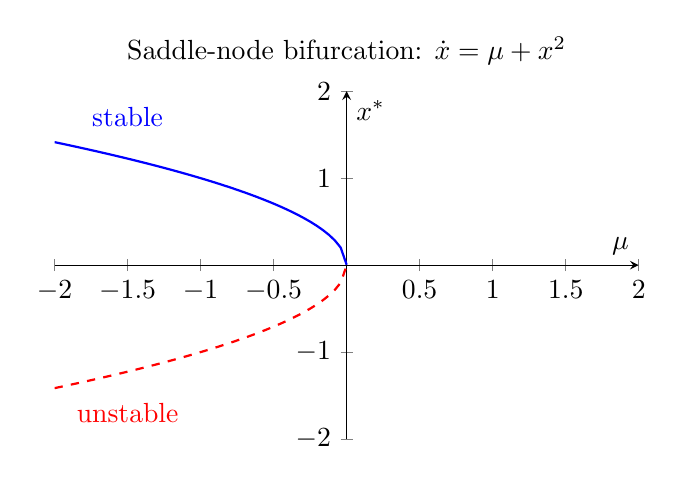
\begin{tikzpicture}
    \begin{axis}[
        width=9cm, height=6cm,
        xlabel={$\mu$}, ylabel={$x^*$},
        xmin=-2, xmax=2, ymin=-2, ymax=2,
        axis lines=middle,
        title={Saddle-node bifurcation: $\dot{x} = \mu + x^2$}
    ]
    \addplot[blue, thick, domain=-2:0, samples=50] {sqrt(-x)};
    \addplot[red, thick, dashed, domain=-2:0, samples=50] {-sqrt(-x)};
    \node[blue] at (axis cs:-1.5,1.7) {stable};
    \node[red] at (axis cs:-1.5,-1.7) {unstable};
    \end{axis}
\end{tikzpicture}
\end{center}

\section{Transcritical Bifurcation}

\begin{definition}[Transcritical bifurcation]
In a \textbf{transcritical bifurcation}, two equilibria exchange their
stability at the bifurcation point, without creation or disappearance.
\end{definition}

\begin{theorem}[Transcritical normal form]
The normal form is $\dot{x} = \mu x - x^2$.
\begin{itemize}
    \item For $\mu < 0$: $x^* = 0$ stable, $x^* = \mu$ unstable.
    \item For $\mu > 0$: $x^* = 0$ unstable, $x^* = \mu$ stable.
\end{itemize}
The two equilibrium branches cross at $\mu = 0$ and exchange stability.
\end{theorem}

\begin{example}[Logistic model with constant harvesting]
The model $\dot{N} = rN(1 - N/K) - H$ exhibits a saddle-node bifurcation
as $H$ increases: beyond a critical threshold, the population collapses.
\end{example}

\section{Pitchfork Bifurcation}

\begin{definition}[Pitchfork bifurcation]
The \textbf{pitchfork bifurcation} occurs in systems possessing a symmetry
$x \mapsto -x$. An equilibrium loses stability and gives birth to two new
equilibria.
\end{definition}

\begin{theorem}[Supercritical pitchfork]
The normal form is $\dot{x} = \mu x - x^3$.
\begin{itemize}
    \item For $\mu \leq 0$: only $x^* = 0$ exists, stable.
    \item For $\mu > 0$: $x^* = 0$ unstable, two new stable equilibria
    $x^* = \pm\sqrt{\mu}$.
\end{itemize}
\end{theorem}

\begin{theorem}[Subcritical pitchfork]
The normal form is $\dot{x} = \mu x + x^3$.
\begin{itemize}
    \item For $\mu < 0$: $x^* = 0$ stable, two unstable equilibria
    $x^* = \pm\sqrt{-\mu}$.
    \item For $\mu \geq 0$: only $x^* = 0$ exists, unstable.
\end{itemize}
The subcritical bifurcation is \textbf{dangerous} because the equilibrium
abruptly loses stability with no local stable alternative.
\end{theorem}

\begin{center}
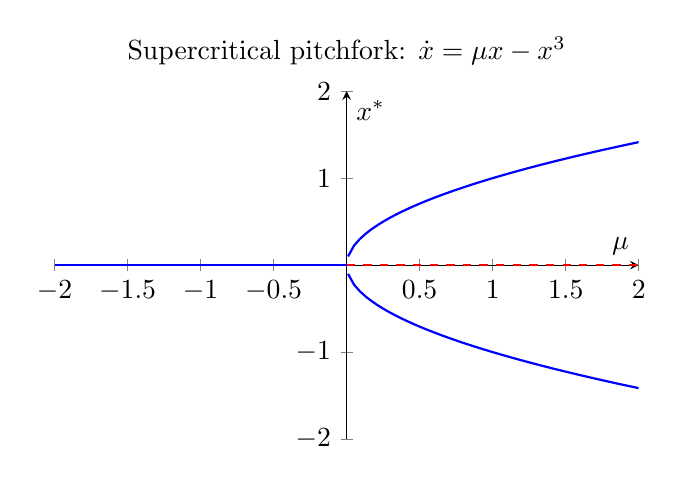
\begin{tikzpicture}
    \begin{axis}[
        width=9cm, height=6cm,
        xlabel={$\mu$}, ylabel={$x^*$},
        xmin=-2, xmax=2, ymin=-2, ymax=2,
        axis lines=middle,
        title={Supercritical pitchfork: $\dot{x} = \mu x - x^3$}
    ]
    \addplot[blue, thick, domain=-2:0, samples=20] {0};
    \addplot[red, thick, dashed, domain=0:2, samples=20] {0};
    \addplot[blue, thick, domain=0.01:2, samples=50] {sqrt(x)};
    \addplot[blue, thick, domain=0.01:2, samples=50] {-sqrt(x)};
    \end{axis}
\end{tikzpicture}
\end{center}

\begin{example}[Euler buckling]
The deflection of a beam under axial load $P$ is governed by
\[
    EI\frac{d^2\theta}{ds^2} + P\sin\theta = 0.
\]
Linearized, this yields a supercritical pitchfork bifurcation at
$P_c = \pi^2 EI / L^2$ (Euler critical load).
\end{example}

\section{Hopf Bifurcation}

\begin{definition}[Hopf bifurcation]
The \textbf{Hopf bifurcation} occurs when a pair of complex conjugate
eigenvalues crosses the imaginary axis. It gives birth to a limit cycle
(or destroys one).
\end{definition}

\begin{theorem}[Hopf]
\label{thm:hopf}
Let $\dot{x} = f(x, \mu)$ with $f(0, \mu) = 0$ for all $\mu$ and
$A(\mu) = D_x f(0, \mu)$ having eigenvalues
$\lambda(\mu) = \alpha(\mu) \pm i\beta(\mu)$. Suppose:
\begin{enumerate}
    \item $\alpha(0) = 0$, $\beta(0) = \omega_0 \neq 0$ (eigenvalues on
    the imaginary axis);
    \item $\alpha'(0) \neq 0$ (transversality condition: eigenvalues cross
    the imaginary axis with nonzero speed).
\end{enumerate}
Then:
\begin{itemize}
    \item \textbf{Supercritical Hopf} (first Lyapunov coefficient
    $\ell_1 < 0$): a \textbf{stable} limit cycle is born for $\mu > 0$
    (the equilibrium becomes unstable);
    \item \textbf{Subcritical Hopf} ($\ell_1 > 0$): an \textbf{unstable}
    limit cycle exists for $\mu < 0$ (the equilibrium is still stable),
    and disappears at $\mu = 0$.
\end{itemize}
\end{theorem}

\begin{keyformulas}[title=\textbf{First Lyapunov coefficient}]
For the system $\dot{z} = (\alpha + i\omega)z + c_1 z\abs{z}^2 + \cdots$
in complex coordinates, the first Lyapunov coefficient is
$\ell_1 = \text{Re}(c_1)$. If $\ell_1 < 0$, the bifurcation is supercritical.
\end{keyformulas}

\begin{example}[Stuart-Landau oscillator]
The model $\dot{z} = (\mu + i\omega)z - z\abs{z}^2$ in polar coordinates
$(r, \theta)$ gives
\[
    \dot{r} = \mu r - r^3, \qquad \dot{\theta} = \omega.
\]
For $\mu > 0$, a stable limit cycle of radius $r = \sqrt{\mu}$ exists.
This is the prototypical supercritical Hopf bifurcation.
\end{example}

\begin{codeblock}[title=\textbf{Bifurcation diagram and Hopf}]
\begin{minted}{python}
import numpy as np
from scipy.integrate import solve_ivp
import matplotlib.pyplot as plt

def hopf_system(t, state, mu):
    x, y = state
    r2 = x**2 + y**2
    return [mu*x - y - x*r2, x + mu*y - y*r2]

fig, axes = plt.subplots(1, 3, figsize=(15, 5))
mus = [-0.5, 0.0, 0.5]
for ax, mu in zip(axes, mus):
    for r0 in [0.1, 0.3, 0.8, 1.5, 2.0]:
        for th in [0, np.pi/2, np.pi, 3*np.pi/2]:
            x0 = [r0*np.cos(th), r0*np.sin(th)]
            sol = solve_ivp(hopf_system, [0, 30], x0,
                            args=(mu,), max_step=0.05)
            ax.plot(sol.y[0], sol.y[1], 'b-', lw=0.3)
    ax.set_title(f"$\\mu = {mu}$")
    ax.set_xlim(-2, 2); ax.set_ylim(-2, 2)
    ax.set_aspect('equal'); ax.grid(True, alpha=0.3)
plt.suptitle("Supercritical Hopf bifurcation", fontsize=14)
plt.tight_layout()
plt.savefig("hopf_bifurcation.pdf")
plt.show()
\end{minted}
\end{codeblock}

\section{Bifurcation Diagrams}

\begin{definition}[Bifurcation diagram]
A \textbf{bifurcation diagram} represents the equilibria (or cycle
amplitudes) as a function of the parameter $\mu$. Stable branches are drawn
as solid lines, unstable branches as dashed lines.
\end{definition}

\section{Global Bifurcations}

\begin{definition}[Homoclinic bifurcation]
A \textbf{homoclinic bifurcation} occurs when a homoclinic orbit (connection
from a saddle to itself) appears or disappears. It can generate a limit
cycle of large period.
\end{definition}

\begin{definition}[SNIC bifurcation]
The \textbf{SNIC} (Saddle-Node on an Invariant Circle) bifurcation occurs
when a saddle-node appears on a limit cycle, destroying it. The period of the
cycle tends to infinity at the bifurcation.
\end{definition}

\begin{theorem}[Period scaling]
\begin{itemize}
    \item SNIC bifurcation: $T \sim \frac{1}{\sqrt{\mu - \mu_c}}$;
    \item Homoclinic bifurcation:
    $T \sim -\frac{1}{\lambda_s}\ln\abs{\mu - \mu_c}$, where $\lambda_s$
    is the stable eigenvalue of the saddle.
\end{itemize}
\end{theorem}

\section{Bifurcations in Higher Dimensions}

\begin{remark}
In dimension $n > 2$, the same local bifurcations occur via center manifold
reduction. The conditions are identical but apply to the reduced system.
Specific bifurcations also appear:
\begin{itemize}
    \item \textbf{Bogdanov-Takens} (codimension 2): double zero eigenvalue;
    \item \textbf{Hopf-Hopf} (codimension 2): two pairs of purely imaginary
    eigenvalues;
    \item \textbf{Cusp} (codimension 2): degeneracy of the saddle-node.
\end{itemize}
\end{remark}

\section{Physical Applications}

\begin{example}[Laser]
A semiconductor laser is modeled by rate equations:
\[
    \dot{n} = J - n - (1 + 2n)P, \qquad \dot{P} = \gamma\left[(1 + 2n)P - P + \beta n\right].
\]
The laser transition (below to above threshold) is a transcritical
bifurcation. In certain models with optical feedback, a Hopf bifurcation
generates oscillations.
\end{example}

\section{Exercises}

\begin{exercise}[Saddle-node in dimension 2]
Study the bifurcations of the system $\dot{x} = \mu - x^2$, $\dot{y} = -y$.
Draw the bifurcation diagram.
\end{exercise}

\begin{exercise}[Pitchfork with imperfection]
Consider $\dot{x} = h + \mu x - x^3$ with $h$ small. Show that the
imperfection $h$ breaks the pitchfork symmetry and draw the diagram in the
$(\mu, x^*)$ plane for $h > 0$.
\end{exercise}

\begin{exercise}[Hopf in a chemical system]
For the Brusselator $\dot{x} = 1 - (b+1)x + ax^2y$,
$\dot{y} = bx - ax^2y$, find the Hopf bifurcation value as a function of
$a$ and $b$.
\end{exercise}

\begin{exercise}[Complete diagram]
For $\dot{x} = \mu x + x^3 - x^5$, draw the complete bifurcation diagram,
identify saddle-node and pitchfork bifurcations, and determine the presence
of hysteresis.
\end{exercise}

\begin{exercise}[Hopf bifurcation --- computation]
Compute the first Lyapunov coefficient for the system
$\dot{x} = \mu x - y - x(x^2 + y^2)$,
$\dot{y} = x + \mu y - y(x^2 + y^2)$
and determine whether the bifurcation is supercritical or subcritical.
\end{exercise}

\begin{exercise}[Homoclinic bifurcation]
Consider the system $\dot{x} = y$, $\dot{y} = x - x^2 + \mu y$. Show that
a homoclinic orbit exists for a particular value of $\mu$ and discuss the
creation/destruction of a limit cycle.
\end{exercise}
